\documentclass[a4paper,11pt,dvipdfmx]{jsarticle}


% 数式
\usepackage{amsmath,amsfonts}
\usepackage{bm}
\usepackage{physics}
\usepackage{mathtools}
% 画像
\usepackage[dvipdfmx]{graphicx}
\usepackage{circuitikz}
\usepackage{amsmath,amssymb}
\usepackage{siunitx}
\usepackage{float}
\usepackage{tikz}
\usepackage{askmaps}
\usepackage{multirow}
\usepackage{bigstrut}
\usepackage{rotating}
\usepackage{listings}
\usepackage{subcaption}
% 表
\usepackage{makecell}
% その他
\usepackage{url}
\usepackage{ascmac}
\usepackage{cases}
\usepackage{here}
\usepackage{upgreek}
\usepackage{tocloft}  % tocloftパッケージを使う
\usepackage{titlesec} % titlesecパッケージを使う(セクションタイトルのカスタマイズ)

% 画像挿入コマンド
\newcommand{\Figure}[4]{
\begin{figure}[H]
\centering
\includegraphics[width=#1\linewidth]{./images/#2}
\caption{#3}
\label{fig:#4}
\end{figure}
}

\begin{document}

\begin{table}[b]
  \centering
  \begin{tabular}{|c|c|}
    \hline
    報告者     & 22120 222 塚田 勇人 \\
    \hline
    共同実験者 & 22192 234 山本 悠介  \\ & 22060 211 古城 隆人\\
    \hline
    担当者     & 楡井 雅巳 \\
              &  藤澤 義範\\
    &力丸 彩奈\\
    &村田 雅彦\\
    &富岡 雅弘\\
    \hline
    実験年月日 & 2024年11月22日 天気:曇り 気温:21.1℃ 湿度38\verb#%#\\
    & 2024年12月6日 天気:曇り 気温:21.8℃ 湿度35\verb#%#\\
    \hline
    提出期限   & 2024年11月21日 17:00  \\
    \hline
    提出日     & \today              \\
    \hline
  \end{tabular}
\end{table}

\title{セレクタ基板のリバースエンジニアリング}
\author{学籍番号:22120 \\ 組番号:222 \\名前:塚田 勇人}
\date{\today}
\maketitle

\newpage

\section{目的}
電子天秤の作成のために,減算基板のリバースエンジニアリングを行い,基板の回路図を作成する.
リバースエンジニアリングとは,製品の作業工程の反対をたどって,製品の構造や仕組みについて考えることである.
そのために,減算基板の動作を確認して,マルチテスタを用いて,実際の回路を探査する.
そして,探査して得られた情報をもとに,回路図を作成する.
その過程を通して,減算基板についての理解を深めることが目的である.

\section{原理}

\section{実験環境}
本実験では,減算基板のリバースエンジニアリングを行う.
減算基板に関する基本的な知識や使われている電子部品について説明する.

\subsection{減算基板} \label{subsec:genzan}
減算基板は,複数の入力信号から1つの信号を選択して出力する基板である.
真理値表を表\ref{tab:selector}に示す.

\begin{table}[H]
  \caption{減算基板の真理値表}
  \centering
  \begin{tabular}{|cc|cc|}
    \hline
    SW0 & SW1 & OUT                     & EN \\
    \hline
    0   & 0   & * & 0  \\
    0   & 1   & B                       & 1  \\
    1   & 0   & C                       & 1  \\
    1   & 1   & A                       & 1  \\
    \hline
  \end{tabular}
  \label{tab:selector}
\end{table}

\subsection{74LSシリーズIC}
今回の実験で用いるICのそれぞれの機能やピンアサインについて説明する.
本実験では,74LSシリーズのICを用いる.
74LSシリーズは,バイポーラトランジスタを用い  て構成されている.

\subsubsection{74LS04}
SN74LS04Nとは,NOTゲートを6つ内蔵したICである.NOTゲートは,入力された信号を反転させる回路である.

\subsubsection{SN74LS08}
SN74LS08Nとは,ANDゲートを4つ内蔵したICである.ANDゲートは,入力された信号がすべてHighのときにHighを出力する回路である.

\subsubsection{SN74LS32}
SN74LS32Nとは,ORゲートを4つ内蔵したICである.ORゲートは,入力された信号のうち1つでもHighがあればHighを出力する回路である.

\subsubsection{SN74LS86}
SN74LS86Nとは,XORゲートを4つ内蔵したICである.XORゲートは,入力された信号が異なるときにHighを出力する回路である.

\subsubsection{HD74LS83AP}
HD74LS83A は,4ビットの2進加算のできる全加算器が内蔵されたICである.
各ビットの和がΣ 出力として得られ,4ビット目の出力からの桁上信号が $C_4$出力に得られる.
5番ピンにVCC,12番ピンにGNDが接続されている.

\subsection{セラミックコンデンサ} \label{subsec:ceramicCapacitor}
セラミックコンデンサは,セラミックを絶縁体として用いたコンデンサである.
このコンデンサは無極性であるため,接続時に極性を気にする必要がない.
主にノイズ処理の役割でバイパスコンデンサとして使用される.


\subsubsection{バイパスコンデンサ} \label{subsec:bypassCapacitor}
バイパスコンデンサとは,回路を誤動作から守るために使用されるコンデンサのことである\cite{digital}.
バイパスコンデンサの接続方法について説明する.
今回の基板に実装されているバイパスコンデンサは,ICの電源端子とGND端子の間に接続されている.
この接続方法には,IC内部のスイッチング時に発生したノイズを外に出さない働きがある\cite{digital}.

\subsection{マルチテスタ}
今回のようにアナログマルチテスタを使用する場合は抵抗値の測定をするときに0ω 調整をする必要がある.
回路の探査をする際には,マルチテスタを導通確認モードにして減算基板の回路の調べたい場所にテスタの端子を当て,どこが導通しているかを確認する.


\section{実験方法} \label{sec:method}
減算基板のリバースエンジニアリングを行うための実験方法について説明する.

\subsection{実験に用いた機器} \label{subsec:equipment}
今回の課題に用いた機器や電子部品について表\ref{tab:equipment}と表\ref{tab:electronicParts}に示す.

\begin{table}[H]
  \caption{実験に用いた機器}
  \centering
  \begin{tabular}{c|c|c}
    \hline
    器具名         & 製造元    & 計器番号    \\
    \hline \hline
    マルチテスター & NISHIZAWA & MODEL 5220  \\
    \hline
    ACアダプタ     & Fksystem  & GF12-US0520 \\
    \hline
    IC取り外し器   & Sunhayato & MODEL GX-3  \\
    \hline
  \end{tabular}
  \label{tab:equipment}
\end{table}

\begin{table}[H]
  \caption{実験に用いた電子部品}
  \centering
  \begin{tabular}{c|c|c|c}
    \hline
    部品名               & 諸元          & 個数 & 部品記号 \\
    \hline \hline
    炭素被膜抵抗         & 1[kΩ ]   & 1    & R1       \\
    \hline
    炭素被膜抵抗         & 10[kΩ ]  & 1    & R2       \\
    \hline
    集積回路(IC)1        & SN74LS04N     & 1    & IC1      \\
    \hline
    集積回路(IC)2        & SN74LS08N     & 2    & IC2~IC3 \\
    \hline
    集積回路(IC)3        & SN74LS32N     & 1    & IC4      \\
    \hline
    集積回路(IC)4        & HD74LS83AP     & 1    & IC5      \\
    \hline
    集積回路(IC)5        & SN74LS86N     & 3    & IC6~IC8 \\
    \hline
    ピンヘッダ           & 2 × 7ピン & 2    & PH1~PH2 \\
    \hline
    LED                  & 赤            & 1    & LED1     \\
    \hline
    セラミックコンデンサ & 0.1[µF]       & 8    & C1~C8   \\
    \hline
  \end{tabular}
  \label{tab:electronicParts}
\end{table}

\subsection{動作確認}
まずは減算基板の動作を調べる.
減算基板のICソケットに場所や向き間違えたり,ICの足を折ったりしないように気をつけながらICをはめ込む.
動作確認用減算基板と動作確認用セレクタ基板,動作確認用入力基板,動作確認用7セグメント,ACアダプタを取り付け,基板の動作を確認する.
接続すると図\ref{fig:zentai}のような回路ができる.そして,減算基板の動作を真理値表にまとめると表\ref{tab:genzan}のようになる.

\Figure{0.5}{全体図.png}{動作確認用基板の接続図}{zentai}

\begin{table}[H]
  \caption{減算基板の真理値表}
  \centering
  \begin{tabular}{|c|c|c|}
    \hline
    入力A,Bの関係 & 出力C & LEDの状態 \\
    \hline
    $A>=B$  & $A-B$   & 点灯    \\
    $A<B$   & $B-A$   & 消灯    \\
    \hline
  \end{tabular}
  \label{tab:genzan}
\end{table}

\subsection{回路の予想}
基板の実際の動作や全加算器,半加算器の回路の知識をもとに,減算基板の回路を予想する.
原始的な半加算器の図を図\ref{fig:halfAdder}に示す.
\Figure{0.4}{HA.drawio.png}{半加算器の図}{halfAdder}

\subsection{回路の探査}
次に,マルチテスタを用いて,減算基板の回路を探査する.
このとき,ACアダプタを外してから探査を行う必要があるので忘れずに行う.
ACアダプタを外すことで短絡事故を防ぐことができる.
また,ICが取り付けてあると調べづらいので,ICをソケットから外して探査を行う.
ICを取り外す際には,IC取り外し器を用いてICをソケットから外す.

\subsection{回路図の作成}
得られた情報をもとに回路図を作成する.
ICの対応するピン番号や部品の接続方法に注意して作成する.

\section{実験結果} \label{sec:result}
リバースエンジニアリングによって得られた情報から作成したセレクタ基板の回路図を図\ref{fig:circuit}に示す.
部品記号は,表\ref{tab:electronicParts}に対応している.
バイパスコンデンサは,それぞれのICの電源端子とGND端子の間に並列に接続されている.

\begin{figure}[H] % 現在の位置に固定
  \centering
  \rotatebox{90}{%
    \begin{minipage}{\textheight} % ページ全体に配置するために高さを使用
      \centering
      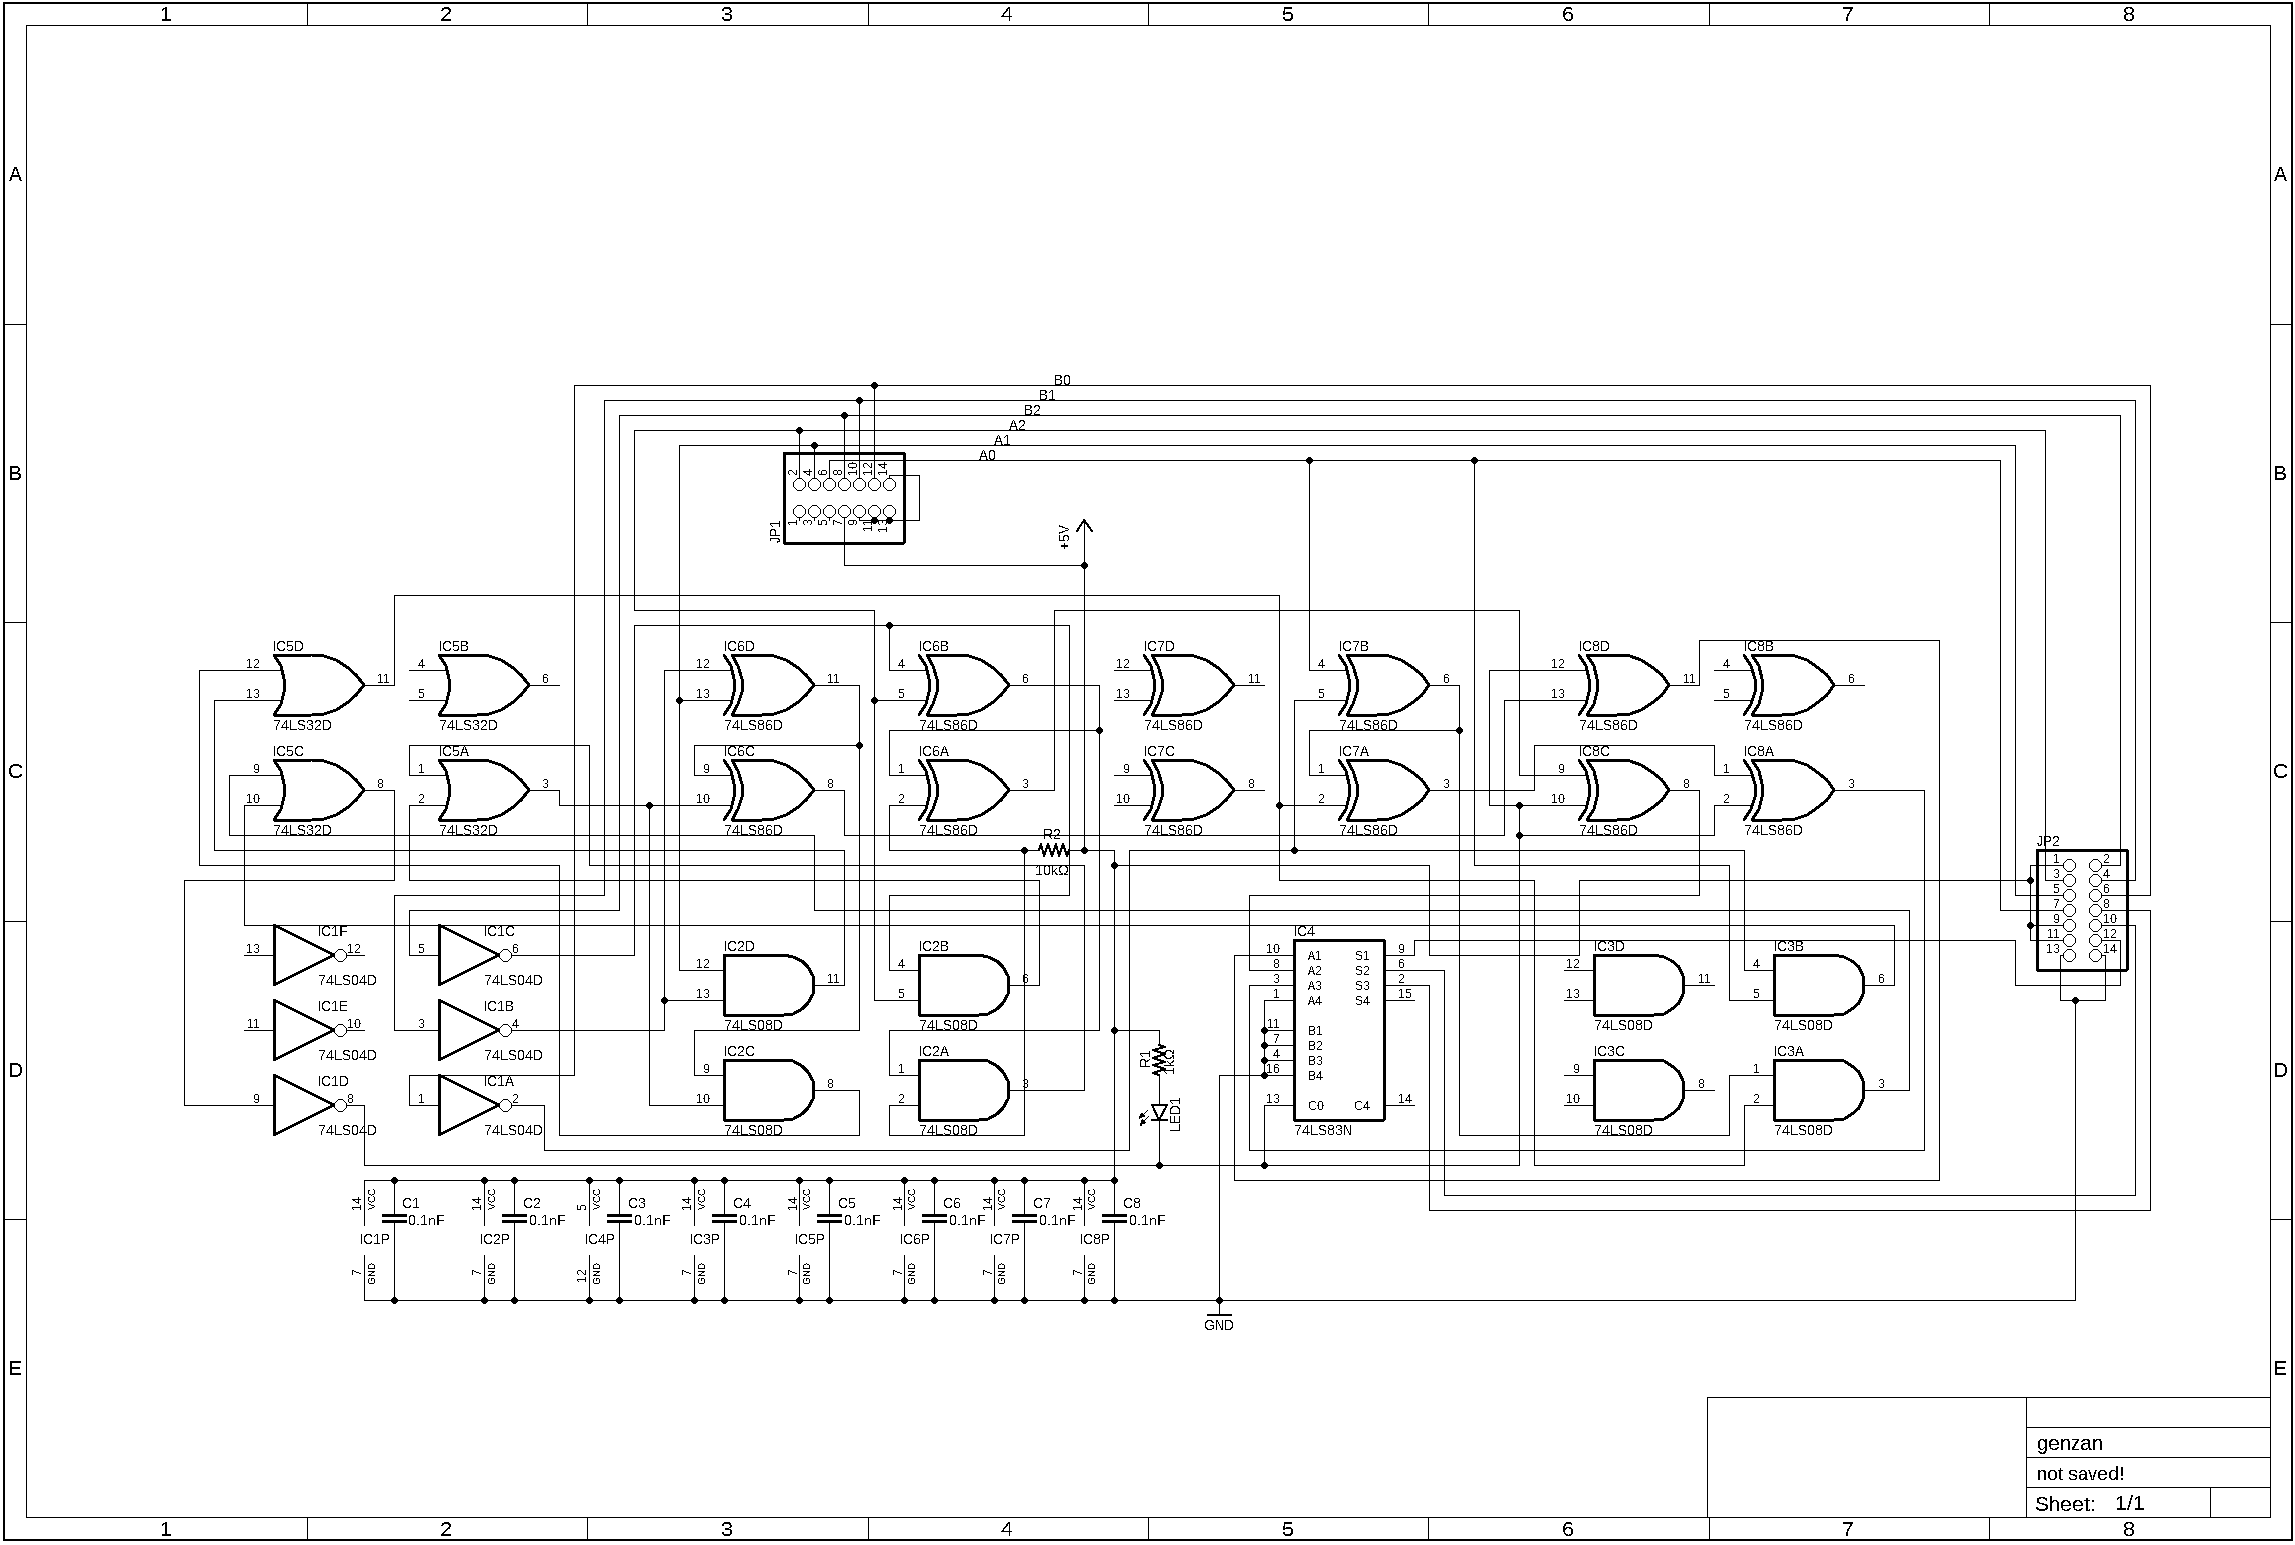
\includegraphics[width=\textwidth]{./images/genzan.png} % 図のサイズを調整
      \caption{減算基板の回路図} % キャプションも回転
      \label{fig:circuit}
    \end{minipage}%
  }
\end{figure}

\section{考察} \label{sec:consideration}
減算基板の動作の確認から,探査を経て回路図を作成することができた.
減算基板のリバースエンジニアリングを通じて,基板の動作や構造を深く理解することができた.
また,マルチテスタを用いた回路の探査の過程では,内部回路の予想と照らし合わせて考えることが非常に有効であった.
リバースエンジニアリングは,電子機器の内部構造を学ぶ上で有効な手法であり,本実験を通して得られた知識は今後の回路設計や電子機器の開発に役立つと考える.


\addcontentsline{toc}{section}{参考文献}
\begin{thebibliography}{99}
  \bibitem{digital}湯山 俊夫 著,『ディジタル回路の設計』,CQ出版株式会社,pp.33-35,(1998年 第19版)
  \bibitem{HD74LS83AP}ルネサス,HD74LS83AP,データシート(2005/06/24)
\end{thebibliography}

\end{document}